\documentclass[fleqn,10pt]{wlscirep}
\usepackage[utf8]{inputenc}
\usepackage[T1]{fontenc}

\usepackage{cite}
\usepackage{amsmath,amssymb,amsfonts}

%\usepackage{tabularx,booktabs}
\usepackage{algorithmic}
\usepackage{multirow, graphicx}
\usepackage{subcaption}
\usepackage{textcomp}
\usepackage{upgreek}
\usepackage{longtable, booktabs}
% \usepackage{arydshln}
\usepackage{afterpage}  % load the afterpage package
\usepackage{color, soul}
%%% HELPER CODE FOR DEALING WITH EXTERNAL REFERENCES
\usepackage{xr}
\makeatletter
\newcommand*{\addFileDependency}[1]{
  \typeout{(#1)}
  \@addtofilelist{#1}
  \IfFileExists{#1}{}{\typeout{No file #1.}}
}
\makeatother

\newcommand*{\myexternaldocument}[1]{
    \externaldocument{#1}
    \addFileDependency{#1.tex}
    \addFileDependency{#1.aux}
}

%
\usepackage{csvsimple}
\usepackage{xstring} % defines \StrDel

\newenvironment{hlbreakable}%
{\color{brown}}%
{}


\usepackage[table]{xcolor} % <---
\usepackage{colortbl}


\usepackage{acro}


\usepackage{pifont}
\newcommand{\cross}{\ding{61} }%
\newcommand{\asterisk}{\ding{87} }%


\DeclareMathOperator*{\argmin}{argmin} % thin space, limits underneath in displays

\graphicspath{{figures/}}
%\RequirePackage{subfig}
\RequirePackage[none]{hyphenat}
\RequirePackage{siunitx}

\RequirePackage{lipsum}
\RequirePackage{xifthen}

%To be able to hide a column in table
\usepackage{array}
\newcolumntype{H}{>{\setbox0=\hbox\bgroup}c<{\egroup}@{}}

\makeatletter
\def\thickhline{%
  \noalign{\ifnum0=`}\fi\hrule \@height \thickarrayrulewidth \futurelet
   \reserved@a\@xthickhline}
\def\@xthickhline{\ifx\reserved@a\thickhline
               \vskip\doublerulesep
               \vskip-\thickarrayrulewidth
             \fi
      \ifnum0=`{\fi}}
\makeatother

\newlength{\thickarrayrulewidth}
\setlength{\thickarrayrulewidth}{5\arrayrulewidth}


%% Acronyms

\DeclareAcronym{tpr}{
  short=TPR,
  long=total peripheral reistance,
}
\DeclareAcronym{bp}{
  short=BP,
  long=blood pressure,
}
\DeclareAcronym{sbp}{
  short=SBP,
  long=systolic blood pressure,
}
\DeclareAcronym{dbp}{
  short=DBP,
  long=diastolic blood pressure,
}
\DeclareAcronym{map}{
  short=MAP,
  long=mean arterial blood pressure,
}
\DeclareAcronym{pe}{
  short=PE,
  long=phenylephrine,
}
\DeclareAcronym{pat}{
  short=PAT,
  long=pulse arrival time,
}
\DeclareAcronym{sqi}{
  short=SQI,
  long=signal quality index,
}
\DeclareAcronym{iqr}{
  short=IQR,
  long=interquartile range,
}
\DeclareAcronym{rmse}{
  short=RMSE,
  long=root mean squared error,
}
\DeclareAcronym{mae}{
  short=MAE,
  long=mean absolute error,
}
\DeclareAcronym{rho_p}{
  short=$\rho_p$,
  long=Pearson's correlation coefficient,
}
\DeclareAcronym{bmi}{
  short=BMI,
  long=body mass index,
}
%%


%
% Reference to the labels and numbers of chapter, section, figures, ...
%

\RequirePackage[noabbrev]{cleveref}
% Default folder for figures
\graphicspath{{figures/}}

\title{Features from the photoplethysmogram and the electrocardiogram for estimating changes in blood pressure - Supplementary Information}

\author[1,*]{Eoin Finnegan}
\author[1]{Shaun Davidson}
\author[1,2,3]{Mirae Harford}
\author[2,3]{Peter Watkinson}
\author[1]{Lionel Tarassenko}
\author[1]{Mauricio Villarroel}
\affil[1]{Institute of Biomedical Engineering, Department of Engineering Science, University of Oxford, UK}
\affil[2]{Critical Care Research Group, Nuffield Department of Clinical Neurosciences, University of Oxford}
\affil[3]{NIHR Oxford Biomedical Research Centre, Oxford, UK.}

\affil[*]{eoin.finnegan@eng.ox.ac.uk}

\renewcommand{\thesection}{SI:~\arabic{section}}
\renewcommand{\thefigure}{SI~\arabic{figure}}
\renewcommand{\thetable}{SI~\arabic{table}}
\renewcommand{\theequation}{SI~\arabic{equation}}
%%%%%%

%Clear page before each section
% \newcommand{\sectionbreak}{\clearpage}

\begin{document}
\maketitlenoabstract

\section{Additional details of PPG principal components features}

\Cref{fig:PCA} shows a visualisation of computed PCA eigenvectors (e.g. the visualisation of PPG PCA 1 is shown as the eigenvector corresponding to the largest eigenvalue in the covariance of $\Psi$\textsubscript{PPG}). %\textcolor{red}{Samples of large amplitude represent regions of interest for that principal component.}

\begin{figure}[h]
	\centering
	\begin{subfigure}{.3\textwidth}
		\centering
		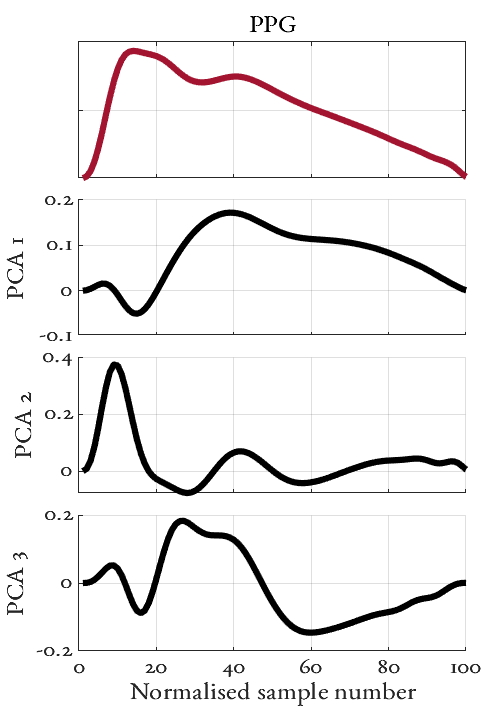
\includegraphics[width = \linewidth]{PCA_component_eigenvectors_PPG.png}
		\caption{}
	\end{subfigure}
	~
	\begin{subfigure}{.3\textwidth}
		\centering
		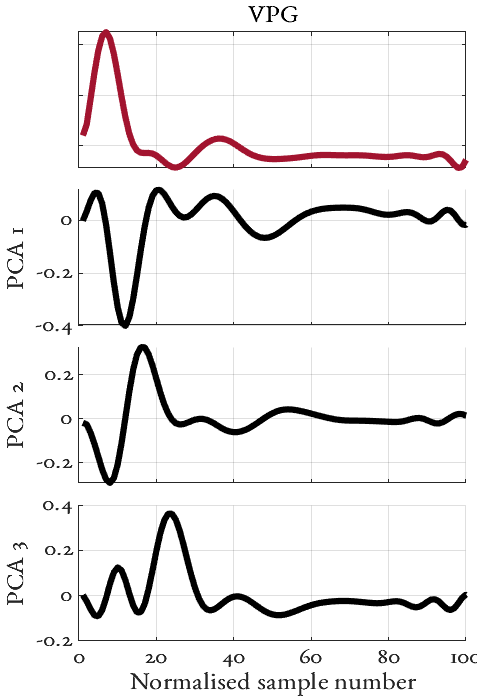
\includegraphics[width = \linewidth]{PCA_component_eigenvectors_VPG.png}
		\caption{}
	\end{subfigure}
	\begin{subfigure}{.3\textwidth}
		\centering
		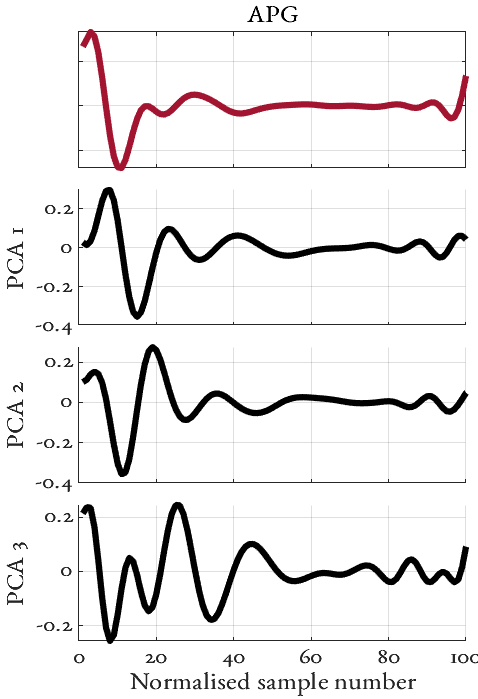
\includegraphics[width = \linewidth]{PCA_component_eigenvectors_APG.png}
		\caption{}
	\end{subfigure}
	\caption{Visualisation of the 3 principal components of the (a) PPG, (b) VPG and (c) APG waveforms using the corresponding eigenvectors. The top row, in red, shows a typical PPG, VPG and APG beat (a-c respectively) in the dataset.}
	\label{fig:PCA}
\end{figure}

\section{Additional details of ECG feature extraction}
\label{sec:ECG_feats_supp}

The following features were extracted from the ECG:

\paragraph{Hjorth parameters}

The Hjorth mobility and complexity parameters indicate activity variations in a signal \cite{Rizal2015}. The mobility parameter represents the signal's mean frequency and is given by: 

\begin{equation}
\text{Mobility} =\sqrt\frac{{\text{var}(\frac{dx(t)}{dt})}}{\text{var}(x(t))}.
\label{eqn:mobility}
\end{equation}
where $x$ is the time series and var($\cdot$) denotes the variance. The signal complexity is an estimate of the signal bandwidth and is given by:
\begin{equation}
\text{Complexity} =\frac{{\text{Mobility}(\frac{dx(t)}{dt})}}{\text{Mobility}(x(t))}.
\label{eqn:complexity}
\end{equation}

\paragraph{Fractal dimension}

The fractal dimension of an ECG signal provides a measure of self-similarity. The fractal dimension of a time series is a number between 1 (straight line) and 2 (defining a surface), where a higher number represents a signal with higher fluctuations and complexity. To calculate the fractal dimension, we used the Higuchi algorithm \cite{Higuchi1988} where increasing length scales (up to $k_{max}$) are used to estimate the signal length. The fractal dimension is then defined as the proportionality constant representing the relationship between length scale and signal length. Brezinski \cite{Brezinski2019} showed that increasing values of $k_{max}$ beyond a value of 17 resulted in only a marginal increase on the fractal dimension for regular ECG beats (defined as an ECG without arrhythmia episodes). Therefore, we set $k_{max}$ as 17 in this work.


\paragraph{Shannon's entropy}

(SE) was used to measure the uncertainty of the information content in a time series based on it's probability distribution. The probability distribution of the time series was estimated by a normalised histogram. SE was then computed as:

\begin{equation}
	\text{SE} = - \sum_{k=1}^{N} p_k \times \text{log}(\frac{p_k}{w_k})
	\label{eqn:shannon_ent}
\end{equation}
where $p_k$ and $w_k$ are the probability and width of the $k^{\text{th}}$ bin of the histogram.

\paragraph{Approximate entropy}
(approxEnt) quantifies the regularity of a time series and the likelihood that similar patterns of observations will not be followed by additional similar observations. For example, a time series containing many repetitive patterns has a small approxEnt. approxEnt was computed using the following steps, and using hyperparamters ($m$ and $r$) defined in \cite{Li2016}:

\begin{enumerate}
\setlength\itemsep{0em}
\item Divide the signal, $x$, of length $N$ into consecutive segments of length $m = 2$
    \item For each segment, $i$, compute the Chebyshev distance to all other segments and calculate $C^{m}_i$ as the number of segments with a Chebyshev distance less than $r = 0.2$ to the $i$\textsubscript{th} segment. 
    \item Define $\phi^{m}(r)$ as the average number of segments of length $m$ that are suitably similar to each other within a tolerance of $r$:
    \begin{equation}
        \phi^{m}(r) = \frac{1}{N-m+1}\sum_{i=1}^{N-m+1}\text{ln}C^{m}_i(r)
    \end{equation}

    \item To compare $\phi^{m}(r)$ to the subsequent data point, increase the dimension to m+1 and compute $\phi^{m+1}(r)$
    \item The approximate entropy is computed as:
    \begin{equation}
        \text{approxEnt}(m, r, N) = \phi^{m}(r) - \phi^{m+1}(r)
        \label{eqn:apprx_ent}
    \end{equation}
\end{enumerate}


\paragraph{Sample entropy}
(sampEnt) is a modification of approxEnt where each segment cannot be compared to itself. In approxEnt, the comparison between each segment and the rest of the segments also includes comparison with itself, as a result signals are interpreted to be more regular than they actually are. These self matches are not included in sampEnt resulting in a more stable estimate of entropy, reducing bias. We computed sampEnt using the same hyperparamters ($m$ and $r$) as approxEnt.


\paragraph{Multi-scale entropy} (MSE) is an extension to sample entropy. MSE is the application of sampEnt to the signal at increasingly coarser scales. For each $s$\textsuperscript{th} scale, the original signal samples are grouped into non-overlapping windows, of length s, and the windowed samples are averaged. sampEnt is then applied to this averaged signal. We computed MSE at scales 2, 4, 6 and 8.


\section{Additional details of cubic smoothing splines to compute the reference BP values}
\label{sec:splines_added_info}

The cubic smoothing splines estimate was computed as follows. First, let a set of observations $y_i$ (in this instance representing BP measurements) at times $t_i$ be modelled by the relation $y_i = f(t_i) + \epsilon_i$ where $\epsilon_i$ are independent, zero mean random variables. Cubic smoothing splines define an estimate, $\hat{f}$, of $f$ that equates to a cubic spline with knots (transition points) at $f(t_i)$. At these transition point, the values of $\hat{f}$, $\hat{f'}$, and $\hat{f''}$ all match. The exact form of $\hat{f}$ is determined by minimising a loss $L^{\text{BP}}$:
\begin{equation}
L^{\text{BP}} = p \sum (y_i - \hat{f}(t_i))^2 + \int \hat{f}''(t)^2 dt
\label{eqn:splines}
\end{equation}
where $p$ is a constant that defines the relative weight placed on minimising the residual sum of squares against the 'roughness' (the accumulated second derivative) of $\hat{f}$. A very low value of $p$ will result in the regressed function converging to a linear least squares estimate. A very high value of $p$ will result in the smoothing spline converging to a cubic spline that passes through all data points. 

As all participants were under the same protocol, we implemented a $p$ value for SBP, MAP and DBP ($p_{\text{SBP}}$, $p_{\text{MAP}}$ and $p_{\text{DBP}}$ respectively) that was common for all of them. Each respective $p$ value was determined by extending the ordinary cross-validation strategy proposed in \cite{Craven1978} by a grid search across the log-scaled range [$10^{-3}$, ..., $10^{8}$]. For each participant, the leave-one-out (LOO) \ac{rmse} was computed across the entire $p$ range. The $p$ value that minimised the participant-wise average LOO error was used.

\newpage
\section{Results for mean arterial pressure and diastolic blood pressure}
\definecolor{TableHeaderBackColor}{rgb}{0.9,0.9,0.9}

\begin{table}[h]
	\caption{Performance statistics of $\Delta$MAP estimation using the models proposed. Results are given as median (IQR) computed across all folds of the LOSOCV. Entries in bold indicate the best performance for that metric.}
	\label{tab:final_results_MAP}
	\centering
	\csvreader[
	tabular={l |c | c| c},
	table head=\hline \rowcolor{TableHeaderBackColor} \textbf{Model name} & \textbf{$\rho_p$} & \textbf{RMSE \textsuperscript{*}} & \textbf{MAE \textsuperscript{*}}\\ \thickhline,
	late after line= \\,
	late after last line= \\  \hline,
    before line=\ifthenelse{\equal{\theFlag}{1}}{\vspace{-10pt} \\ \hline }{},
	head to column names,
	]
	{csv/MAP_results.csv} 
	{}
	{\modelName\textsubscript{\dataName} & \RMed \quad (\RIqr)  & \RmseMed	\quad (\RmseIqr) & \MaeMed \quad (\MaeIqr)}
	\caption*{\textsuperscript{*} results given in units of mmHg}
\end{table}

\begin{table}[h]
	\caption{Performance statistics of $\Delta$DBP estimation using the models proposed. Results are given as median (IQR) computed across all folds of the LOSOCV. Entries in bold indicate the best performance for that metric. }
	\label{tab:final_results_DBP}
	\centering
	\csvreader[
	tabular={l |c | c| c},
	table head=\hline \rowcolor{TableHeaderBackColor} \textbf{Model name} & \textbf{$\rho_p$} & \textbf{RMSE \textsuperscript{*}} & \textbf{MAE \textsuperscript{*}}\\ \thickhline,
	late after line= \\,
	late after last line= \\  \hline,
    before line=\ifthenelse{\equal{\theFlag}{1}}{\vspace{-10pt} \\ \hline }{},
	head to column names,
	]
	{csv/DBP_results.csv} 
	{}
	{\modelName\textsubscript{\dataName} & \RMed \quad (\RIqr)  & \RmseMed	\quad (\RmseIqr) & \MaeMed \quad (\MaeIqr)}
	\caption*{\textsuperscript{*} results given in units of mmHg}
\end{table}



\section{Feature results}

\Cref{tab:collinear_features} provides a summary of all features remaining after removing collinear features. \Cref{fig:Ranking_coeffs_appendix} shows mean ranking coefficients for both (a) RF and (b) LASSO feature importance. 

\def\tablecaption{Resulting features from removing collinearity and their correlated features ($|\rho_p|$ > 0.8, $p$ < 0.05). $\rho_p$\textsubscript{$\Delta$SBP}: correlation to $\Delta$ SBP across all participants, $p$: resulting p value. Features are ordered by their mean RF ranking coefficient. As demographics were included as static variables to the feature set, their correlations are not included. }



\def\tableheadcorr{\hline \rowcolor{TableHeaderBackColor}  \textbf{Feature name} & \textbf{Correlated features} & \textbf{$\rho_p$\textsubscript{$\Delta$SBP}} & \textbf{$p$ }& \textbf{PWC\newline{[q1, q3]}}\\ \hline}

\small{
\csvreader[
longtable={p{3cm} | p{5cm}|cc| >{\centering\arraybackslash} m{2cm} },
  table head=\caption{\tablecaption\label{tab:collinear_features}} \tableheadcorr
  \endfirsthead 
  \hline \multicolumn{5}{r}{\textit{Continued on next page}} \\ \endfoot 
  \caption*{PWC: participant-wise correlation, q1 and q3 show the first and third quartile values, indicating the spread of PWC in the cohort. }
  \endlastfoot
  \multicolumn{5}{c}{\tablename\ \thetable\ -- \textit{Continued from previous page}} \tableheadcorr \endhead,
  late after line= \\,
  late after last line=\hline ,
  head to column names,
  ]
{csv/collinear_results.csv}
{}
{\FeatName & \CorrelatedFeatures & \corrBp & \pBpString  & {[\qone, \qthree]}}
}



\begin{figure}[h]
	\centering
	\begin{subfigure}{.49\textwidth}
		\centering
		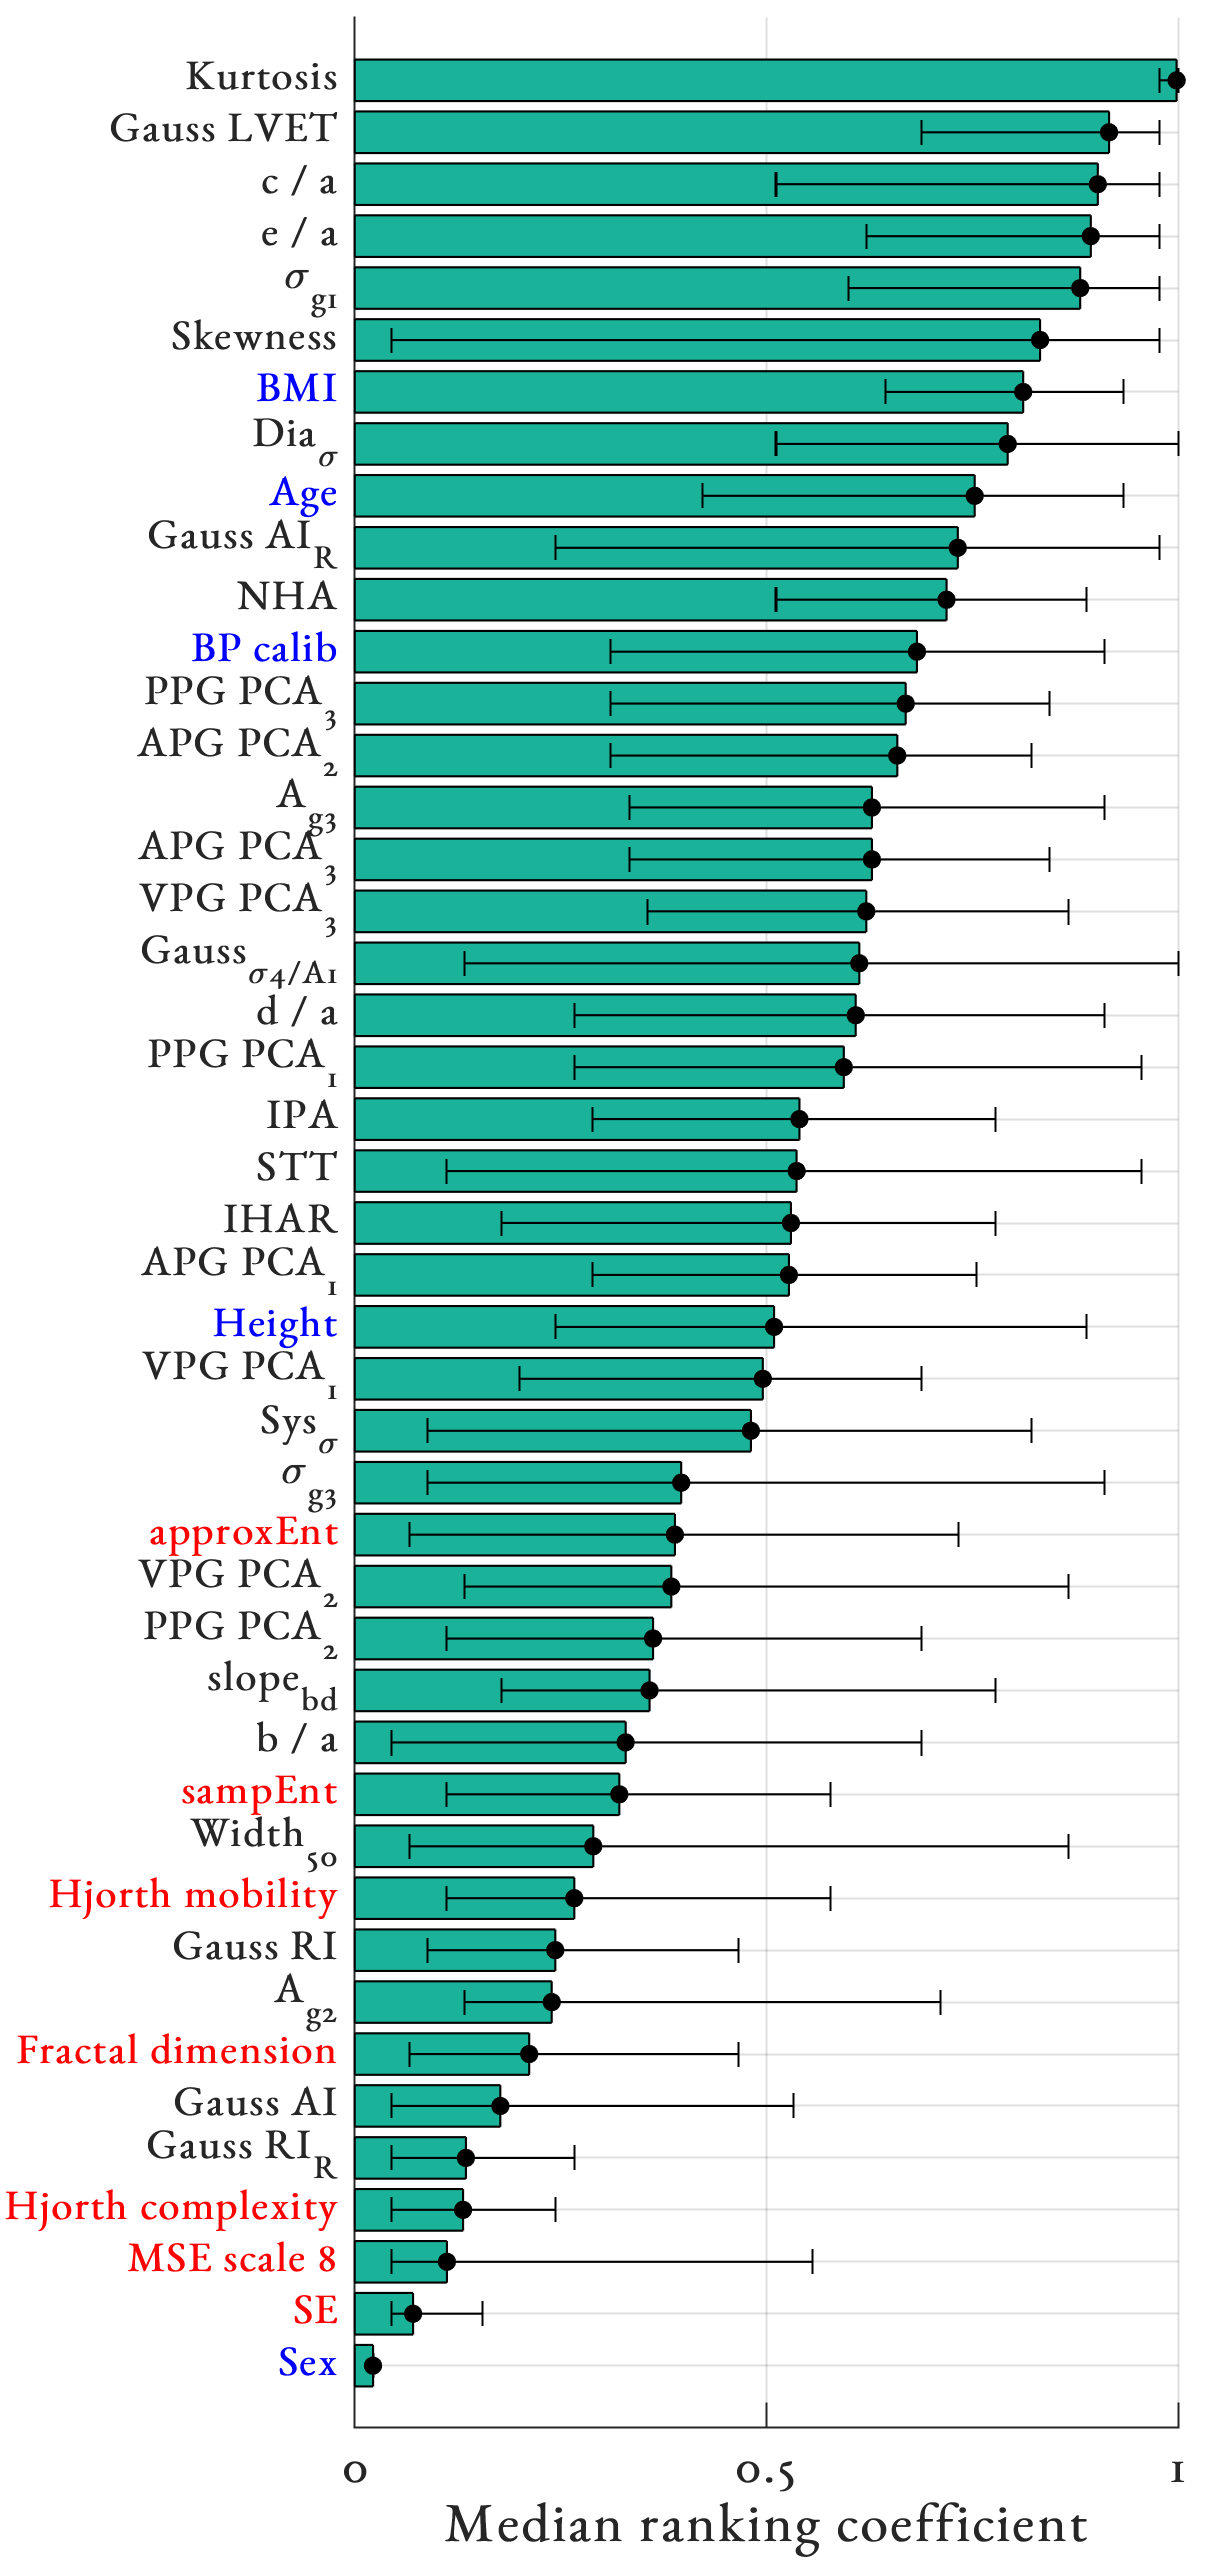
\includegraphics[height = 16cm]{feature_results_RF.png}
		\caption{}
	\end{subfigure}
	~
	\begin{subfigure}{.49\textwidth}
		\centering
		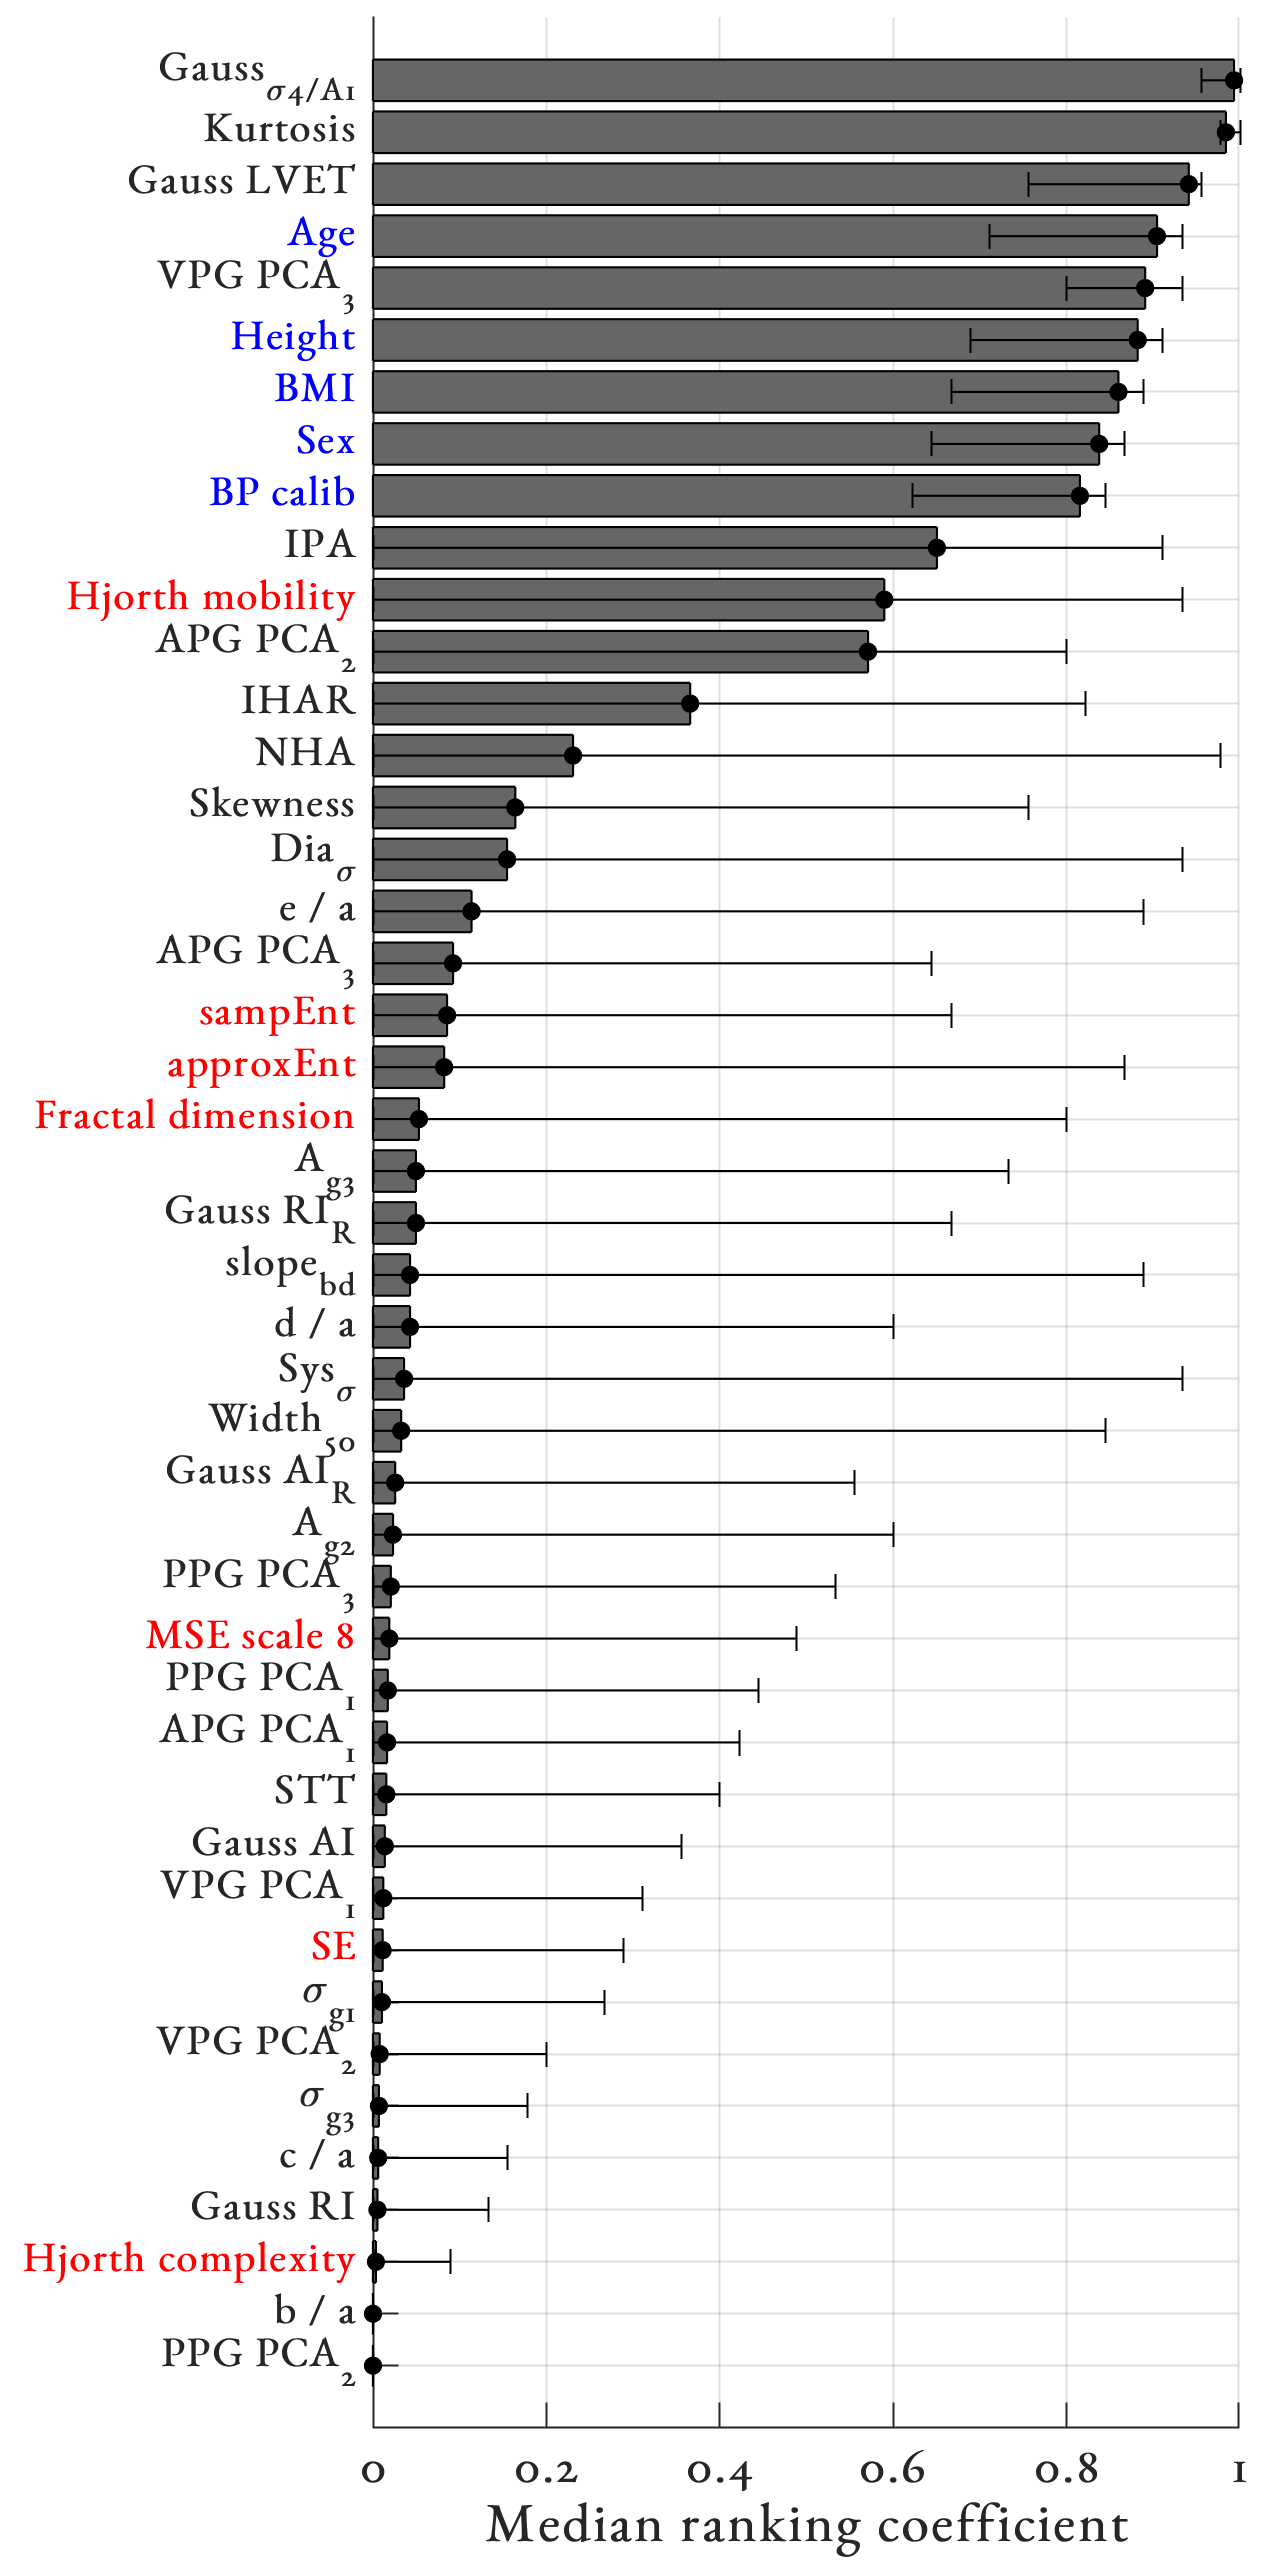
\includegraphics[height = 16cm]{feature_results_LR.png}
		\caption{}
	\end{subfigure}
	\caption{Median ranking coefficient for (a) random forest and (b) LASSO feature importance. Features are ordered by their respective median ranking coefficient. Demographic features are highlighted in blue and ECG features in red for clarity.}
	\label{fig:Ranking_coeffs_appendix}
\end{figure}

\clearpage
\section{Individual results}



\begin{figure}[h!]
	\centering
	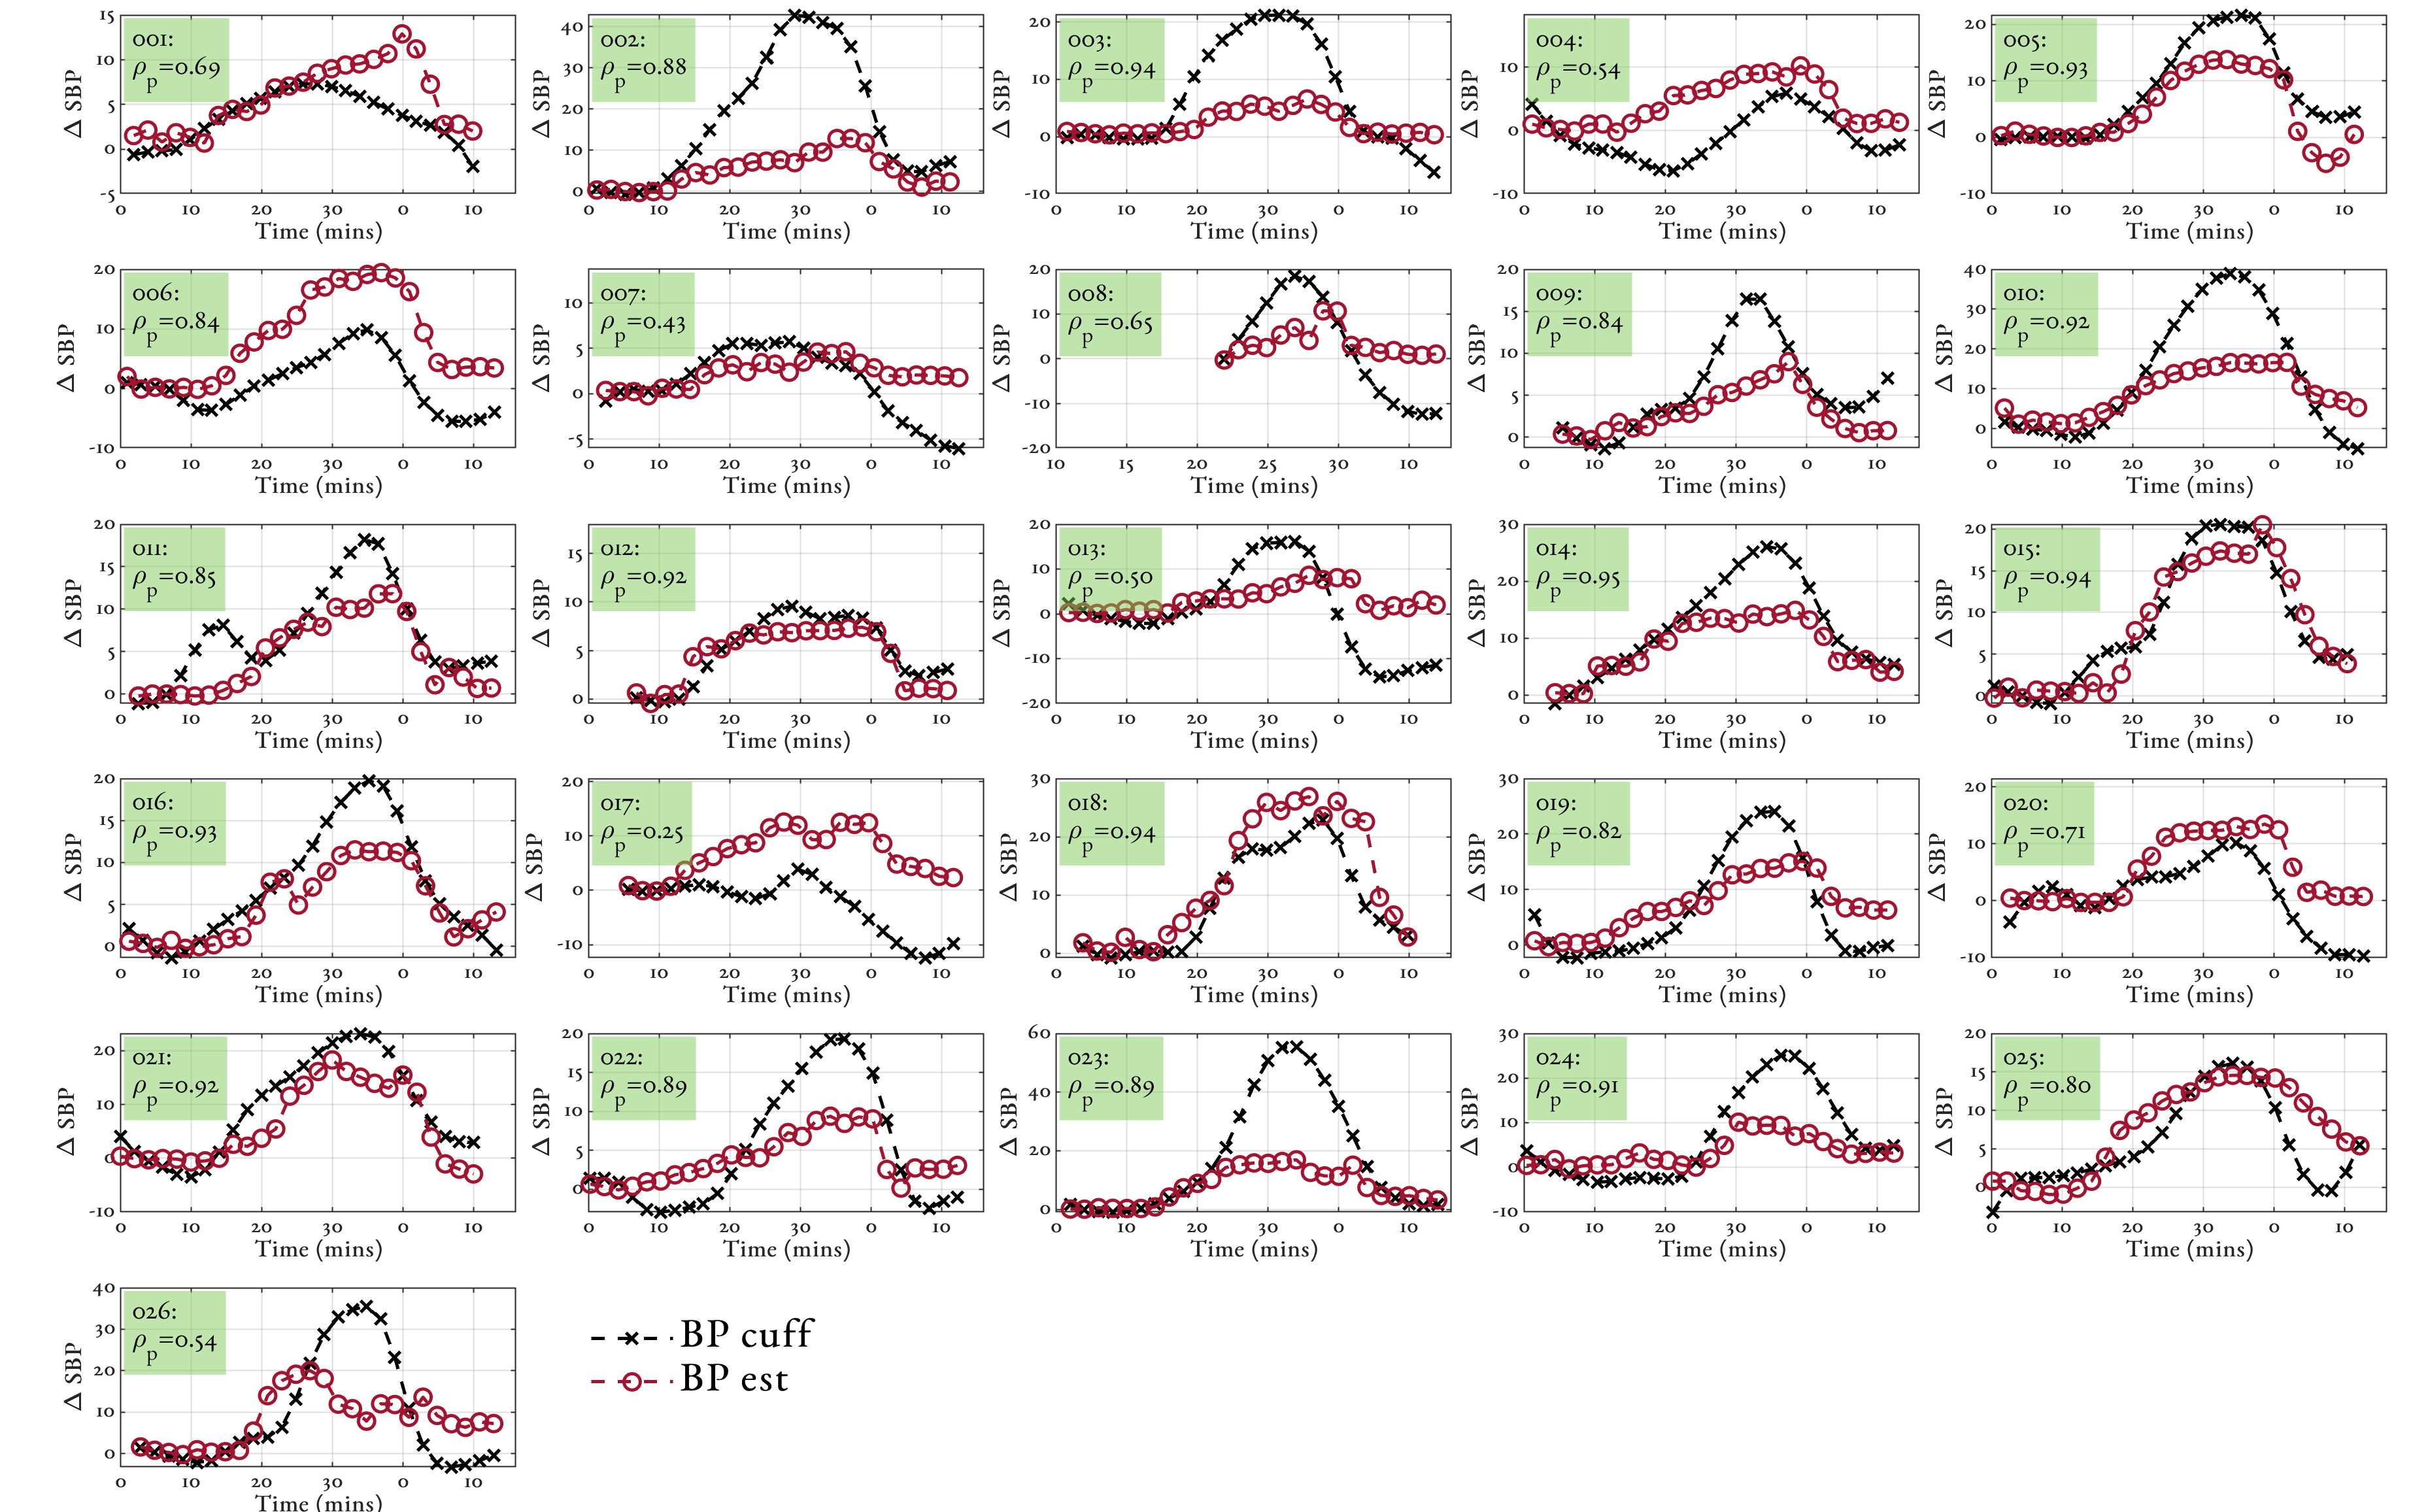
\includegraphics[width = \textwidth]{Individual_results_SBP.png}
	\caption{Individual results of $\Delta$SBP estimation using the RF\textsubscript{PPG + ECG} model across all participants in the study. Note the differences in the y-axis. The reference $\Delta$ SBP values from the cuff are shown in black and the estimated values are shown in red.}
	\label{fig:Individual_results_SBP}
\end{figure}


\begin{figure}[h!]
	\centering
	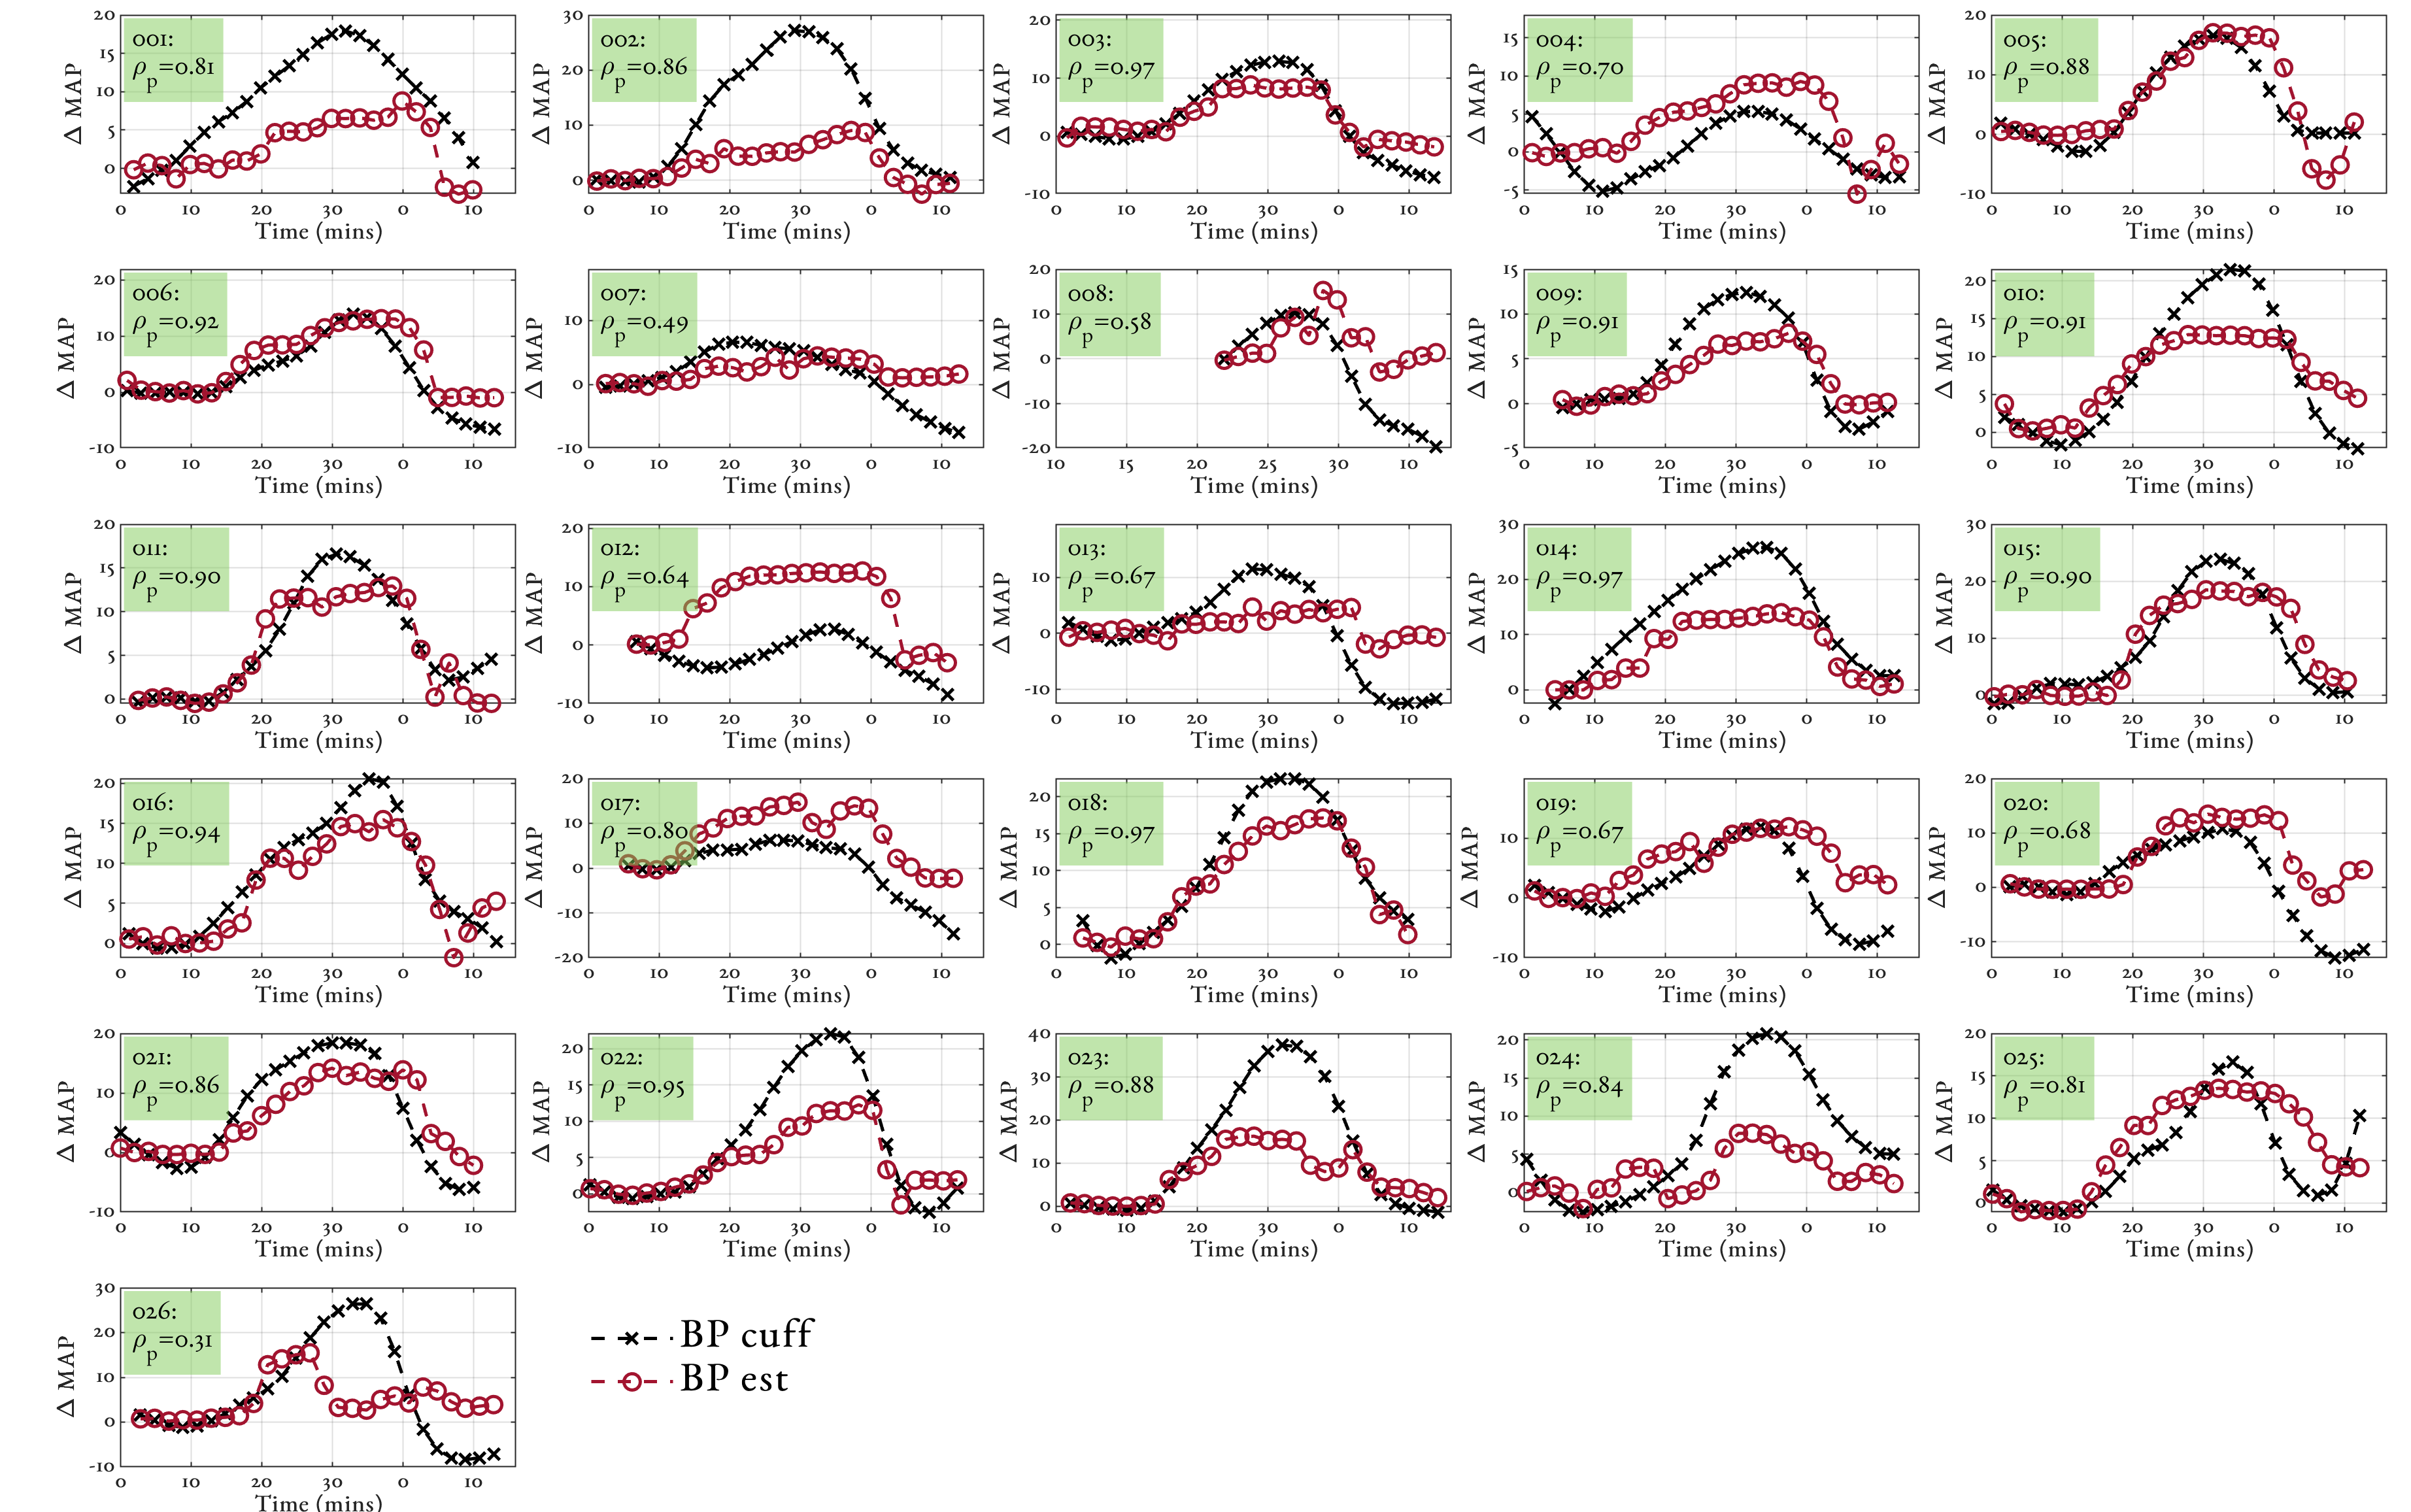
\includegraphics[width = \textwidth]{Individual_results_MAP.png}
	\caption{Individual results of $\Delta$MAP estimation using the RF\textsubscript{PPG + ECG} model across all participants in the study. Note the differences in the y-axis. The reference $\Delta$ MAP values from the cuff are shown in black and the estimated values are shown in red.}
	\label{fig:Individual_results_MAP}
\end{figure}



\begin{figure}[h!]
	\centering
	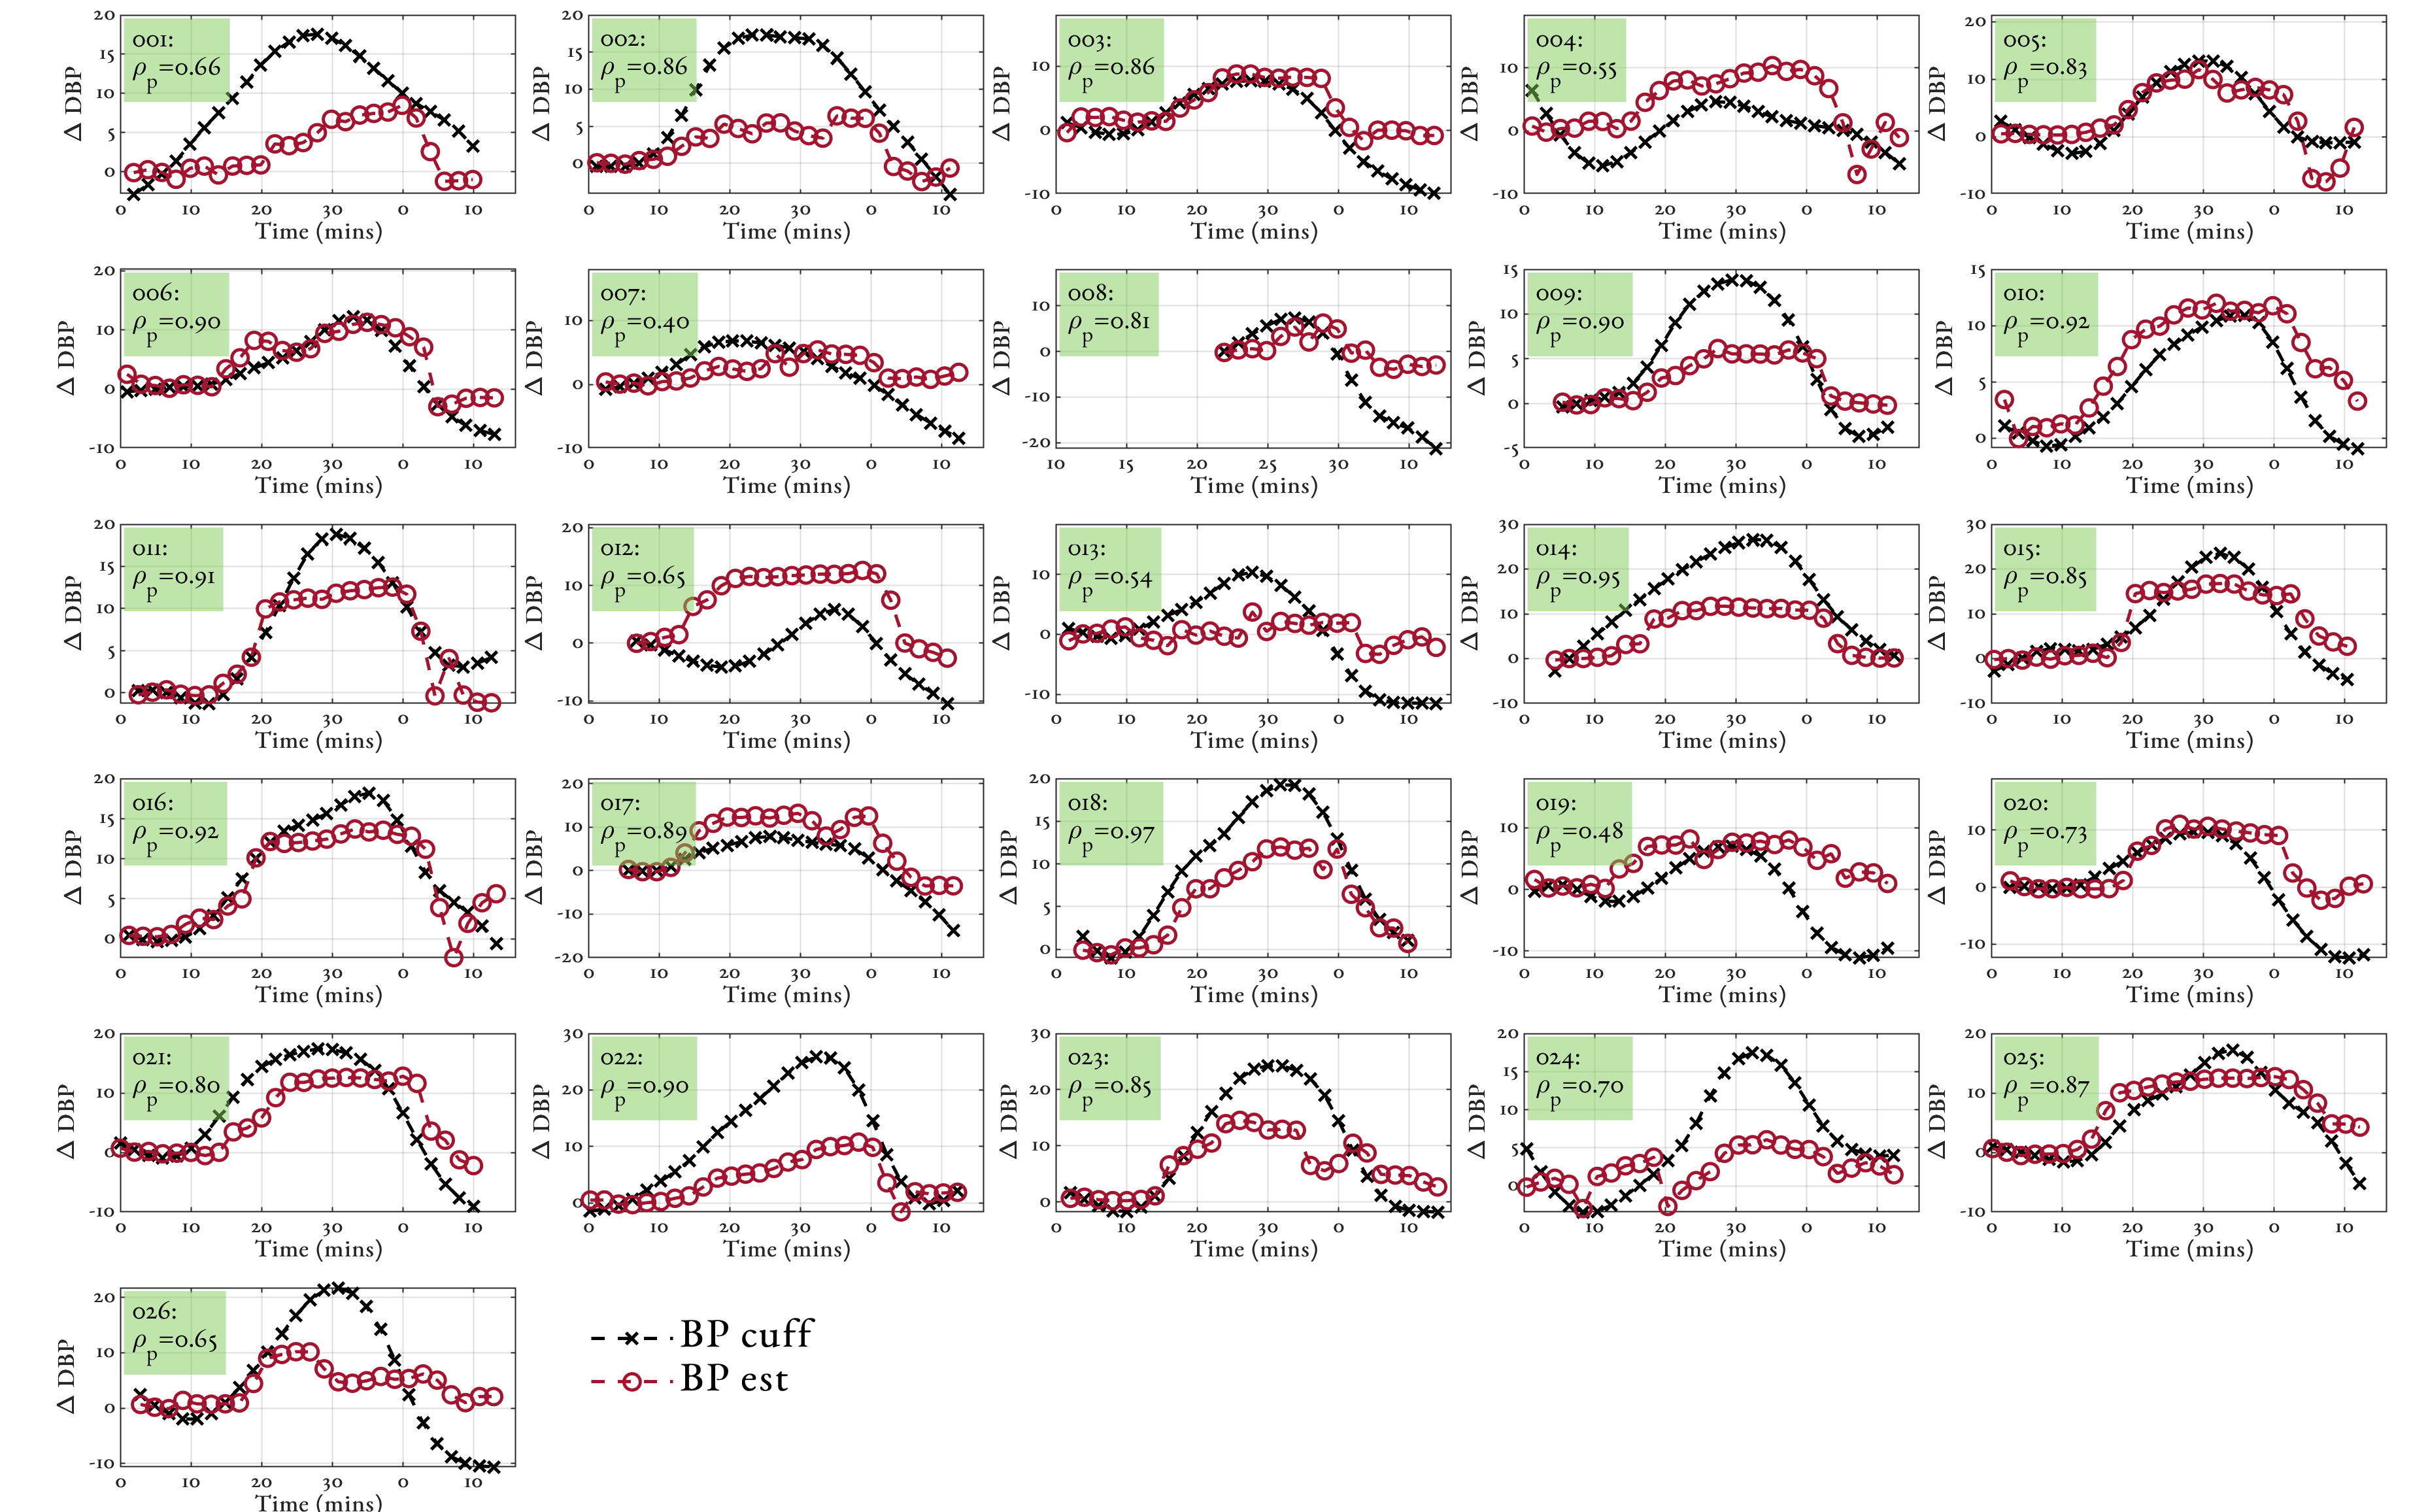
\includegraphics[width = \textwidth]{Individual_results_DBP.png}
	\caption{Individual results of $\Delta$DBP estimation using the RF\textsubscript{PPG + ECG} model across all participants in the study. Note the differences in the y-axis. The reference $\Delta$ DBP values from the cuff are shown in black and the estimated values are shown in red.}
	\label{fig:Individual_results_DBP}
\end{figure}


\clearpage
\section{Individual changes in cardiac output}

\Cref{fig:Individual_results_CO} shows the changes in cardiac output (CO) observed for all individuals in the dataset across the full duration of their session. The majority of individuals experienced a decrease in CO driven by a decrease in HR.

\begin{figure}[h!]
	\centering
	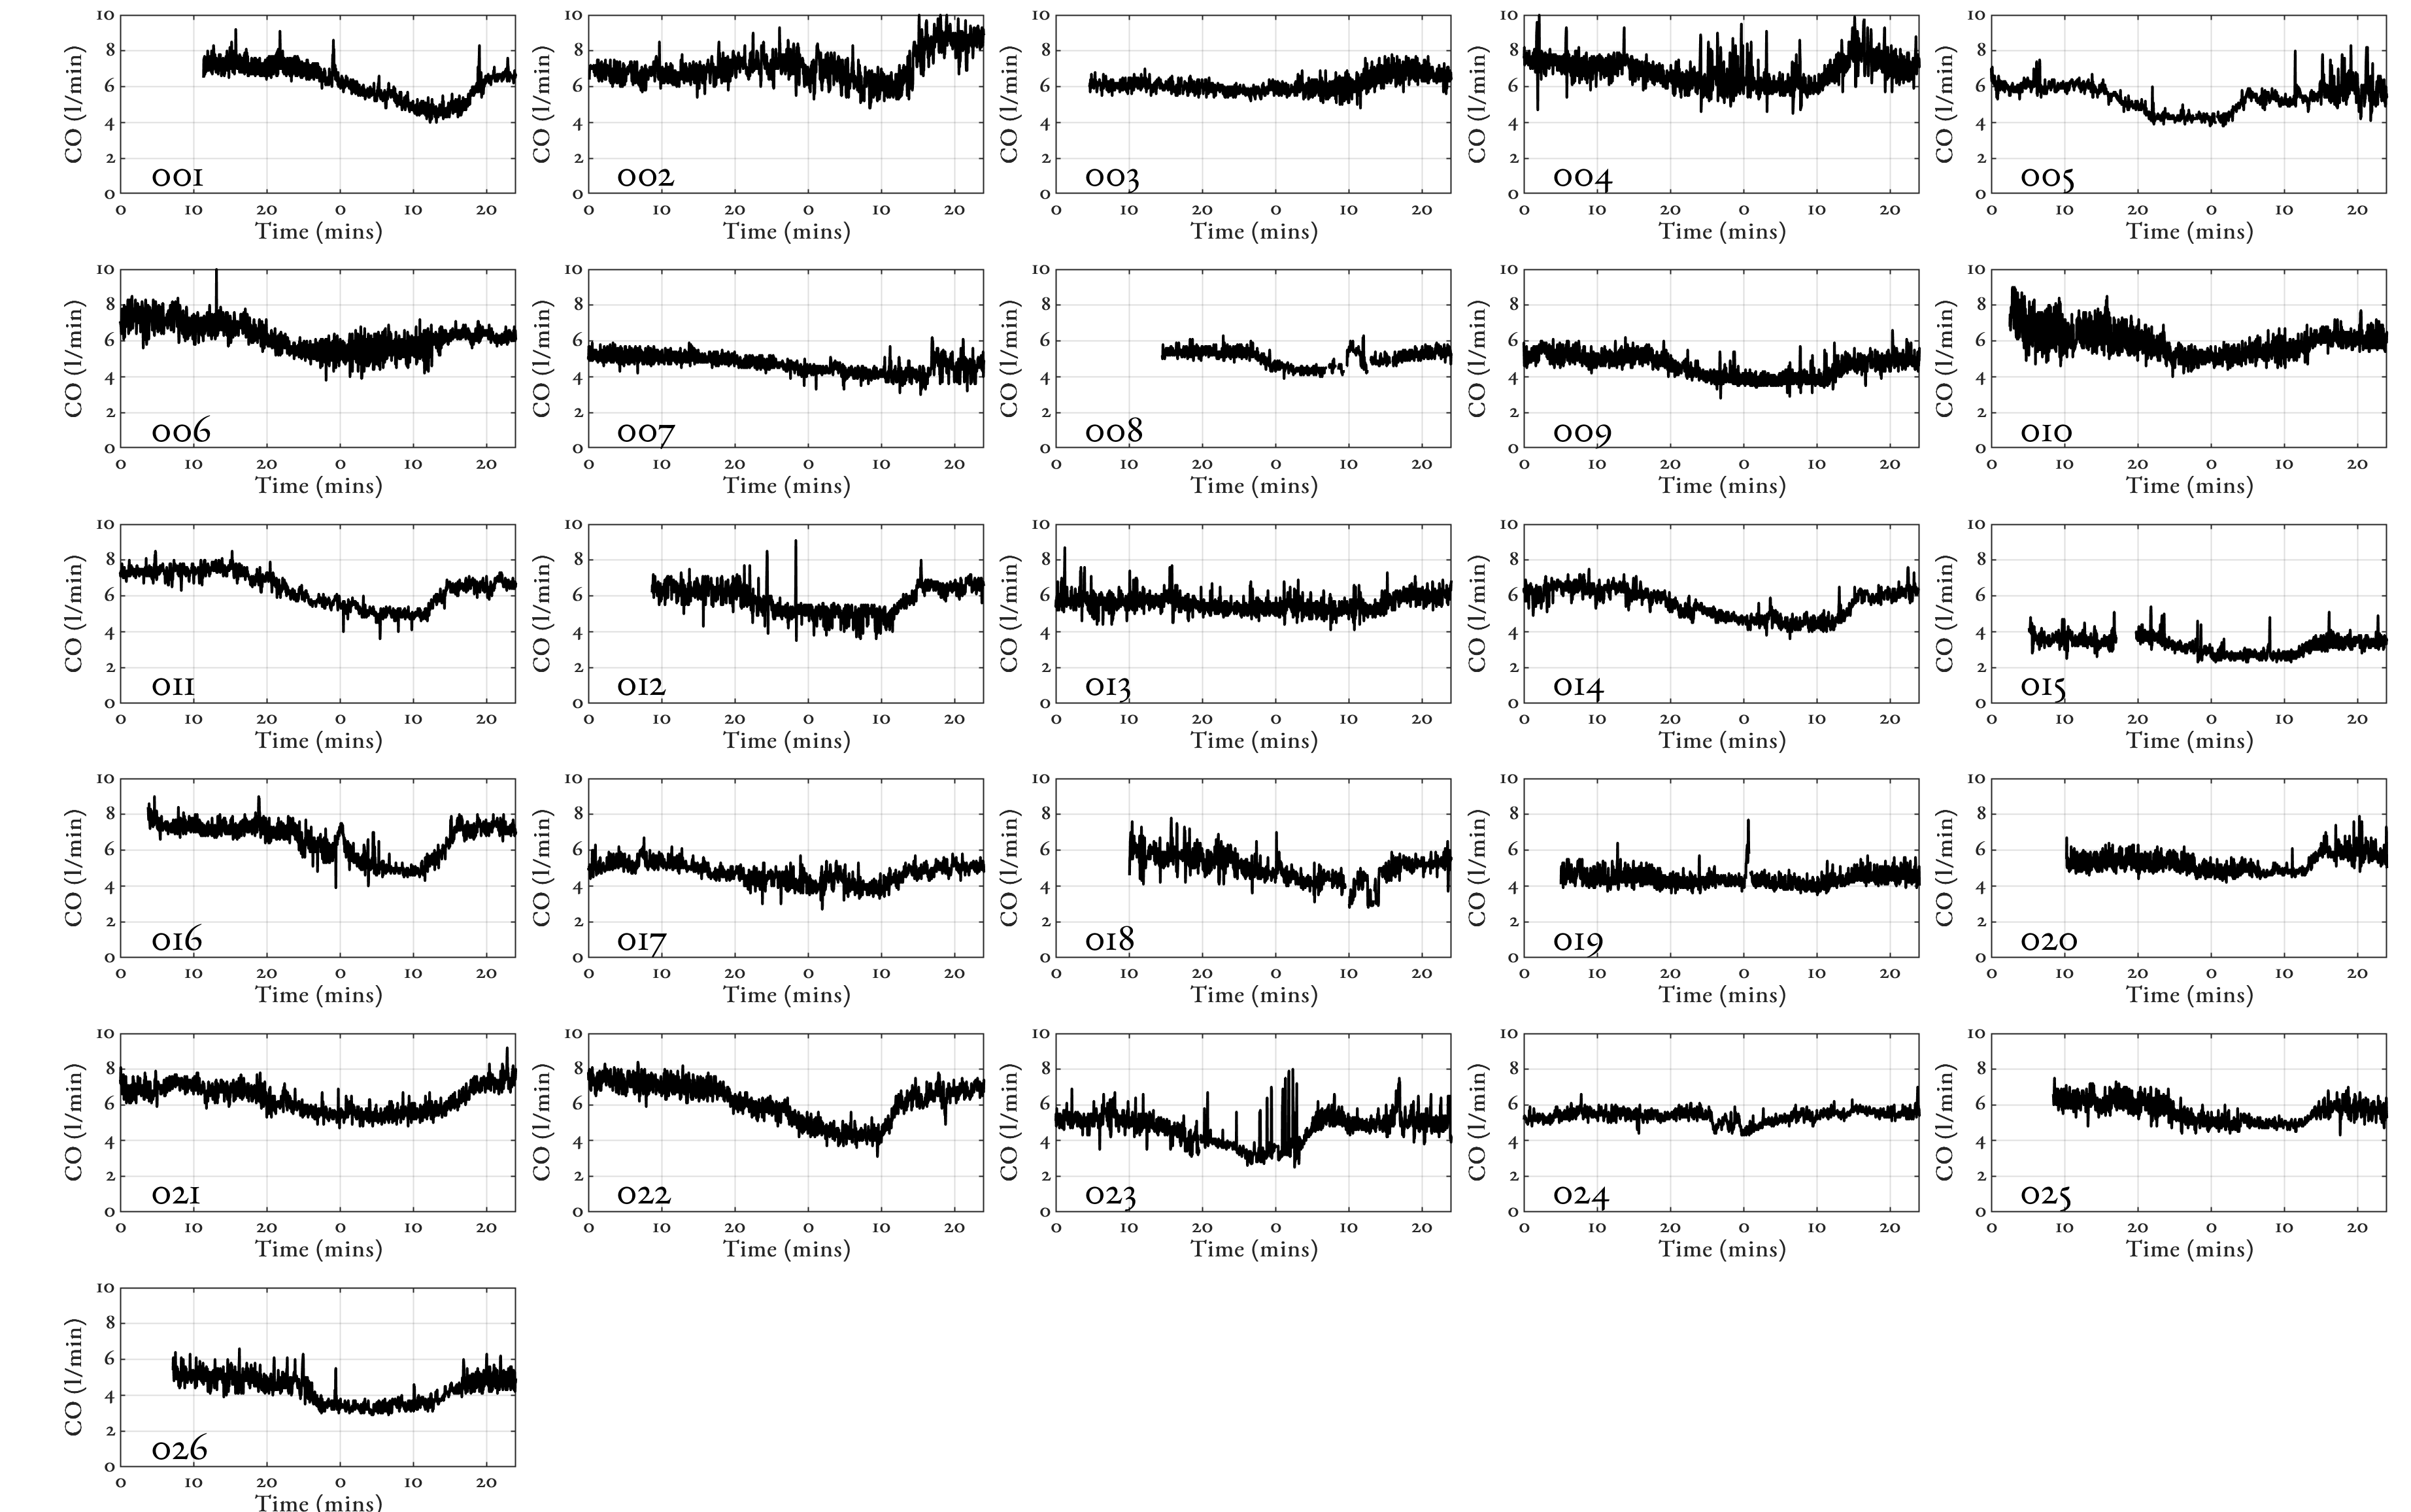
\includegraphics[width = \textwidth]{CO_profiles.png}
	\caption{Individual changes in CO observed in all individuals across the full duration of their session.}
	\label{fig:Individual_results_CO}
\end{figure}



\bibliographystyle{IEEEtran}
\bibliography{references}

\end{document}